\chapter{The Camera Module}

Cameras capture images, and they are the interface between images and
the real world.  This relationship is fundamental in computer vision
algorithms, which are distinguished by the fact that they will tie the
processed pixel data to objects in the real world for the purposed of
measurement, tracking, or display.  This is achieved by modeling the
geometric and physical properties of the device that was used to
capture the original image.  This is the purpose of the camera module.

The camera module includes several built-in models for pinhole and
line-scan imagers and a set of generic functions for linearizing
(removing lens distortion) and epipolar rectifying (e.g. for stereo)
camera models where these operations are relevant.  These classes and
functions can be imported into your code by including {\tt
  <vw/Camera.h>}.  

The camera module is also designed to be extensible: the user can
provide their own camera model by inheriting from the {\tt
  CameraModel} abstract base class in {\tt
  <vw/Camera/CameraModel.h>}. 

Finally, the camera module provides a basic set of tools for working
with images from real-world camera systems: bayer pattern filtering
and EXIF parsing.  We will cover all of these features in more detail,
however we begin this chapter by establishing some terminology while
exploring what is perhaps the most ubiquitous camera geometry in use
today: the pinhole camera model.

\section{The Pinhole Camera Model}
The pinhole camera model should be familiar to you.  This is the
camera geometry that appears in nearly all commercial digital camera
systems today.  It is characterized by a lens assembly that focuses
light onto a two dimensional array of pixels (usually a densely packed
array of light sensitive circuits on a CCD or CMOS device).  We will
use the pinhole model to establish some terminology that will be used
throughout the rest of this chapter.  Be warned that this model is
somewhat simplistic; many of the non-ideal characteristics of a
real-world optical system (e.g. lens distortion) are not modeled in
this simple example, so this model would probably not be a good camera
model on its own.  Refer to the CAHVOR model in Section
\ref{sec:cahvor} for a pinhole camera model that more accurately
models lens distortion.

\subsection{Perspective Projection}

Figure \ref{fig:pinhole} shows the geometry of a basic pinhole camera.
The light gray area represents the 2D array of pixels, and it is
referred to as the {\bf image plane}.  The origin of the 3D coordinate
system is the point $C$, which is the center of projection or {\bf
  camera center} of the imager.  When a 3D point $O$ is imaged by the
camera, it appears at the pixel located where segment $\overline{OC}$
intersects the image plane at point $(u,v)$.  A line segment
$\overline{OC}$ that is perpindicular to the image plane intersects
this plane at the {\bf principal point}, $(p_u, p_v)$.

\begin{figure}[tbp]
\begin{center}
  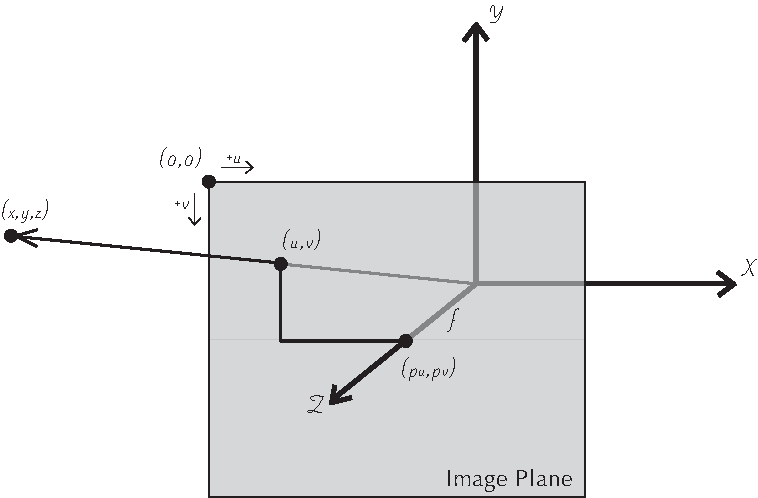
\includegraphics[width=5in]{images/camera_module_pinhole.pdf}
 \end{center}
  \label{fig:pinhole}
  \caption{The basic pinhole camera model.}
\end{figure}

All of the points imaged by the camera appear on a line that passes
through $C$.  If the coordinates of ${\bf O}$ are $(x,y,z)$, then the
position of the point on the imager can be determined by projecting it
onto the plane $ z = +f$:
\begin{eqnarray}
\label{eqn:forward-projection-1}
u &=& \frac{f}{\sigma} \left(\frac{x}{z}\right) - p_u \\
\label{eqn:forward-projection-2}
v &=& \frac{f}{\sigma} \left(\frac{-y}{z}\right) - p_v
\end{eqnarray}

Here, $f$ is the focal length of the imager in meters, $\sigma$ is the
size of a pixel in {\em m/pixel}, and $(p_u, p_v)$ are the offset in
pixels of the principal point (this offset moves the origin of the
image from the principal point to the upper left hand corner, which is
the ``origin'' usually adopted when indexing images).  

Equations \ref{eqn:forward-projection-1} and
\ref{eqn:forward-projection-2} consitute the {\bf forward projection}
portion of the camera model.  They take a 3D point and ``image'' it:
they tell you exactly what what pixel location to look for if you
wanted to see the point $O$ in the image.  

Notice how some information is lost during forward projection.  Any
point along $\overline{OC}$ will be imaged to the same point $(u,v)$
on the image plane, so if we were to start with a point $P=(u,v)$ on
the image plane, and we wanted to find the original 3D point $O$, the
best we could do would be to say that it appears somewhere along the
ray $\overrightarrow{CP}$. The
origin and direction of the ray can be computed as follows:

\begin{eqnarray}
\label{eqn:reverse-projection-1}
\overrightarrow{CP}_{origin} & = & C \\
\label{eqn:forward-projection-2}
\overrightarrow{CP}_{direction} & = & \frac{(u + p_u, -(v + p_v), f)} {||(u + p_u, -(v + p_v), f)||_2};
\end{eqnarray}

Despite the ambiguity in the actual postion of $O$, this operation,
which we call {\bf reverse projection} can still provide useful
inforamation that can be used in a full 3D reconstruction. Imagine
that you have two cameras that have imaged the same point $O$ from two
different viewpoints at pixel locations $P_1$ and $P_2$ respectively.
You could reconstruct the position of $O$ by computing the
intersection of the two rays emanating from each camera center through
$P_i$.  This technique is called stereo vision, and it is one of the
many ways in which you can make use of the information provided by
reverse projection.

\subsection{The Camera Model Base Class}

As we have seen, a camera model provides a means for {\em forward
  projection} (``imaging'' 3D points onto a 2D array of pixels) and
{\em reverse projection} (finding the ray along which a 3D points must
lie given a 2D pixel where it was imaged).  All camera models in the
Vision Workbench derived from the CameraModel abstract base class,
which enforces this basic interface.    

To forward project a 3D point, one calls:

\begin{verbatim}
  CameraModel* camera_model = <some derived camera model class>;  
  Vector2 pixel_coordinates = camera_model.point_to_pixel(world_coordinates);
\end{verbatim}

Remember that in C++, you will need to maintain a pointer to the
derived camera model class in order to ensure that the virtual
inheritance mechanism calls the method from the derived class rather
than the base class.

As we learned in the previous section, this operation of {\em reverse
  projection} can be used to determine the origin and direction of the
ray that passes through the 3D point $O$ that was imaged at pixel
location $(u,v)$.  Any of the points that lie along this ray would
have been imaged at $(u,v)$, so this pixel-to-ray operation leaves
some ambiguity about the true location of the point $O$.

The camera model interface for computing this ray is split into two
stages: (1) finding the origin of the ray (the camera center) and (2) finding
it's direction.

\begin{verbatim}
  CameraModel* camera_model;  
  Vector3 ray_origin = camera_model.camera_center(pixel_coordinates);
  Vector3 ray_direction = camera_model.pixel_to_vector(pixel_coordinates);
\end{verbatim}

\begin{center}\fbox{\parbox{7in}{
{\bf Camera Coordinate Systems}\\ 
\\
Camera models take and return coordinates that are {\em not}
homogeneous.  Homogeneous coordinates, where the vector is augmented
with an additional scaling element usually set to 1 (e.g. a 2D vector
$(325 206)$ in cartesian coordinates will be represented as $(325 206
1)$ in homogeneous coordinates.  Homogeneous coordinates have certain
advantages in projective geometry (e.g. they allow a tranlation of the
coordinates to be encoded as a matrix multiplication), however we have
chosen not to adopt this convention here so as to conserve space and
to provide a simple, unified camera model interface. }}
\end{center}

\subsection{Built-in Camera Models}

Several camera models come ``built-in'' to the Vision Workbench camera
module.  These classes can be used to provide functionality out of the
box, or they can serve as a design reference for your own camera
model.  Each models a specific geometry, and to varying extents they
will also model the non-ideal characteristics of the camera system
such as lens distortion.  

The list of built-in models are summarized in Table
\ref{tab:camera-models}.  The following sections describes the two
basic classes of built-in camera model: those that model pinhole
cameras (where the imager is a 2D array of pixels), and those that
model linescan cameras (where the imager is a 1D line of pixels).

\begin{table}[tdp]
\begin{center}
\begin{tabular}{|l|l|l|l|}
\hline
{\em Camera Model} & {\em Header File} & {\em Imager Type} & {\em Details}\\
\hline CAHV         & {\tt CAHVModel.h} & Pinhole     & Basic pinhole camera model \\
CAHVOR       & {\tt CAHVORModel.h} & Pinhole     & Models lens distortion\\
Linear Pushbroom    & {\tt LinearPushbroomModel.h} & Linescan & Assumes linear flight path \\
Orbiting Pushbroom & {\tt OrbitingPushbroomModel.h} & Linescan & Models curvature of orbit \\
\hline
\end{tabular}
\end{center}
\label{tab:camera-models}
\caption{Built-in camera models can be found in {\tt vw/Camera/} }
\end{table}

\subsubsection{Pinhole Cameras}

The {\em CAHV camera model} has been widely used in NASA planetary mission
for rover navigation and scientific camera systems
\cite{yakimovsky78}.  It is a basic pinhole camera model: it does not
model lens distortion or other optical aberrations.  The CAHV model is
so named because the camera intrinsic and extrincsic parameters are
jointly parameterized by four 3-dimensional vectors: C,A,H, and V.
This compact represenation leads to a very efficient forward
projection operation, and this is the strength of the CAHV model.
Forward projection of a real world point $O$ can be computed using

\begin{eqnarray}
u & = & \frac{(O-C) \cdot H}{(O-C) \cdot A}\\
v & = & \frac{(O-C) \cdot V}{(O-C) \cdot A}
\end{eqnarray}

The user has two choices when initializing a CAHV camera model.
First, they can construct the object by directly supplying four
3-vectors to the constructor.

\begin{verbatim}
  Vector3 C,A,H,V;
  CameraModel* cam = new CAHVORModel(C,A,H,V);
\end{verbatim}

Users seeking to use the CAHV class as a general purpose pinhole
camera model may find it easier to use the more verbose constructor
where the camera extrinsics and intrinsics are explicitly supplied.

\begin{verbatim}
  double focal_length;
  Vector2 pixel_size;
  double principal_point_h, principal_point_v;
  Vector3 camera_center, pointing_vector;
  Vector3 horizontal_vector, vertical_vector;

  CameraModel* cam = new CAHVORModel(focal_length, pixel_size, principal_point_h, 
                                     principal_point_v, camera_center, 
                                     pointing_vector, horizontal_vector,
                                     vertical_vector);  
\end{verbatim}


The {\em CAHVOR camera model} contains two additional 3-vectors (O and R)
that extend the basic CAHV model by adding terms to account for
distortion introduced by the camera lens.

See the API documentation for more information about constructing CAHV
and CAHVOR camera models.

\subsubsection{Linescan Cameras}

Linescan imagers capture images using a sensor containing a single
1-dimensional array of pixels.  The image is formed by capturing
scan-lines with this sensor in rapid succession as the camera platform
is rotated or moved.  A flat-bed scanner or photocopier is an example
of a linescan system that should be familiar.  The sensor is swept
{\em along-track} across the document, composing the final image by
concatenating several thousand adjacent 1-dimensional images taken at
evenly spaced positions.

Linescan sensors are fairly uncommon in commercial camera systems, but
they do appear on satellites that capture photographs of terrain from
orbit.  The orbital motion of the satellite is used in much the same
way as the motion of the sensor in the scanner; the {\em across-track}
dimension of the image corresponds to the projection of 3D points
through the lens onto the sensor, but the along-track dimension of the
image is a function of time as the satellite moves.  

\begin{figure}[tbp]
\begin{center}
  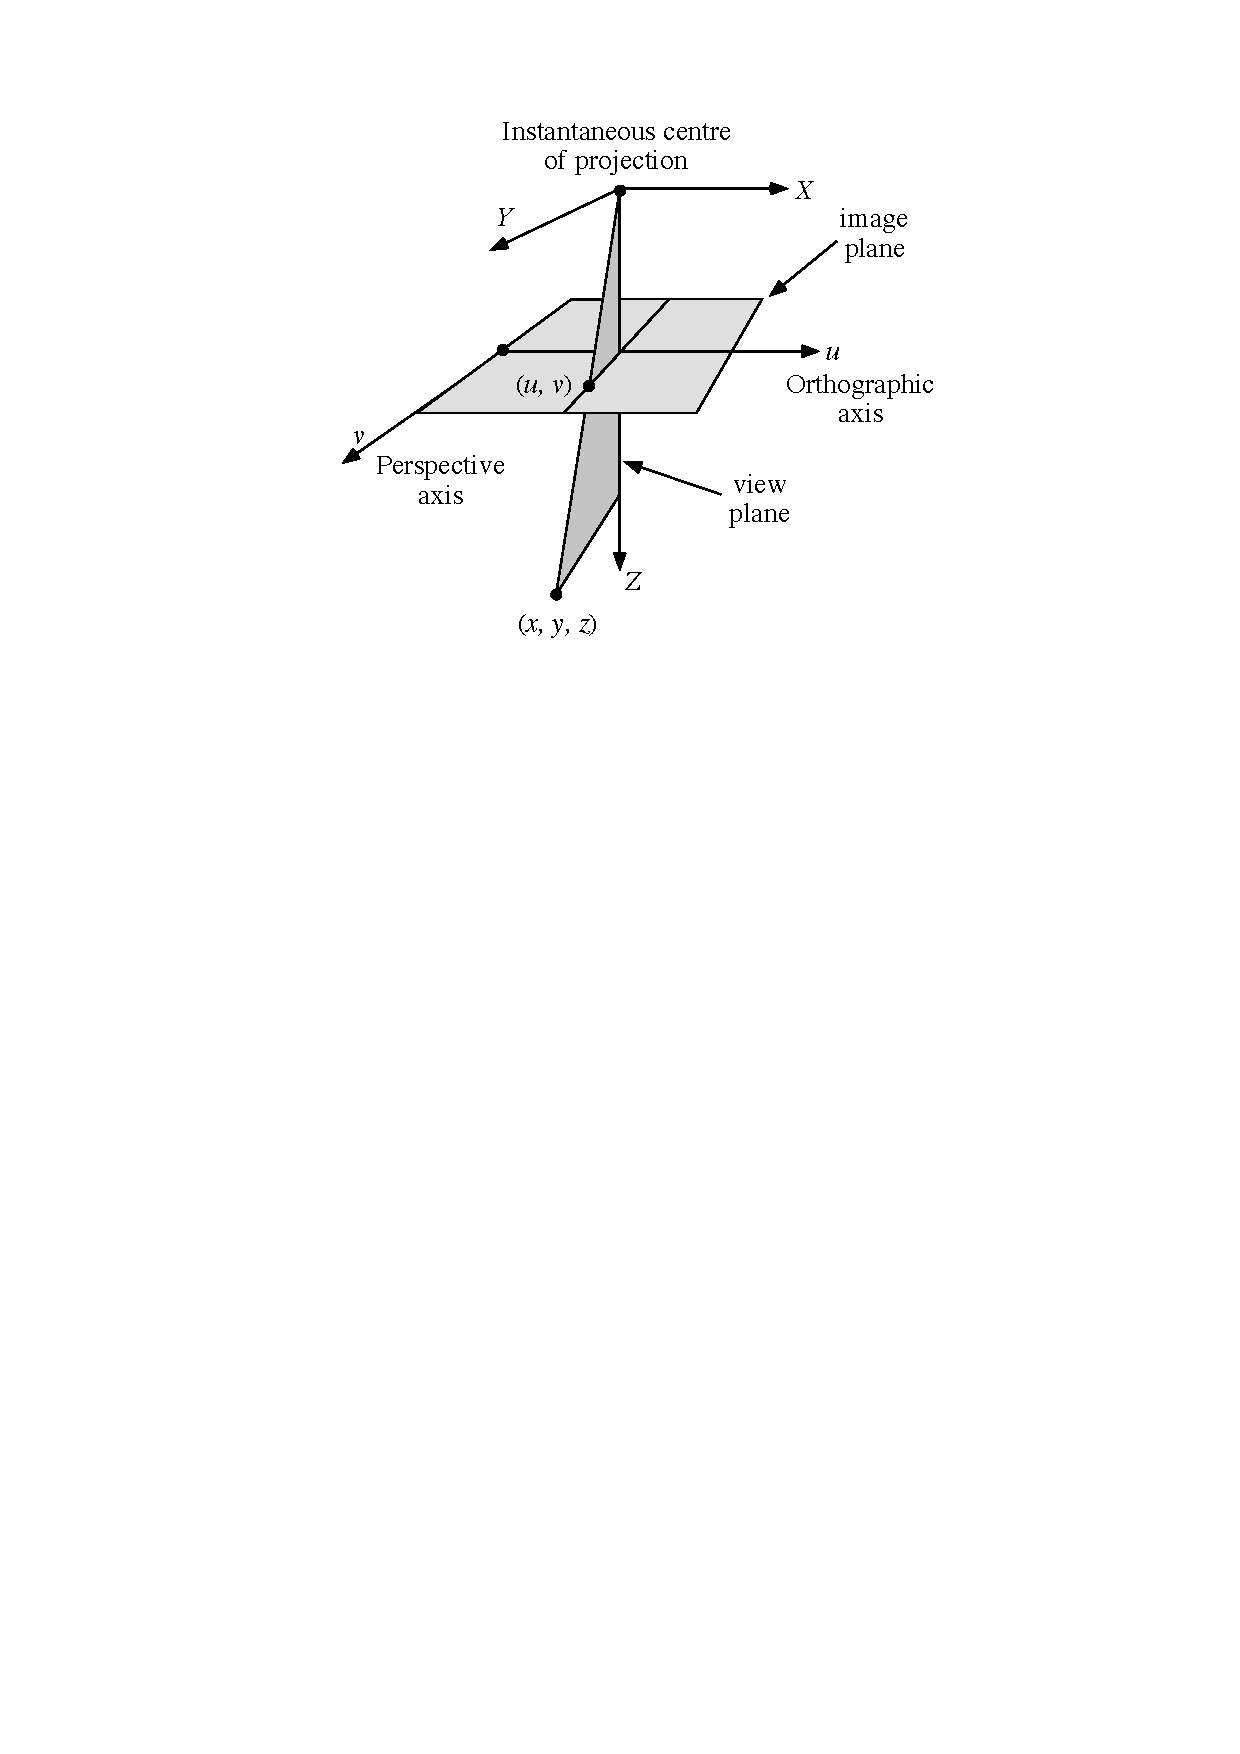
\includegraphics[width=5in]{images/pushbroom_geometry.pdf}
 \end{center}
  \label{fig:pinhole}
  \caption{Geometry of the Linear Pushbroom Camera Model.  Credit:
    Rajiv Gupta and Richard Hartley \cite{gupta97}.}
\end{figure}

The geometry of the linescan imager is subtly different from the
geometry of the pinhole camera.  See Figure \ref{fig:pushbroom}.
Although there is still a center of projection created by the camera's
optics (and points are still imaged using a perspective projection in
the across-track direction), this point moves as the camera moves.  As
a result, the along-track position of a pixel in a linescan image is
purely a function of the extrinsic parameters of the camera: it's
position and orientation, both a function of time.  

In the special case where the motion of the linescan sensor is linear
and its orientation is fixed, the projection of the points onto the
image in the along-track is orthographic.  These assumptions are the
basis for the {\em Linear Pushbroom Model}.  

If you must relax these assumptions somewhat to allow the sensor pose
to vary and the motion to be curved, the {\em Orbiting Pushbroom
  Model} is an appropriate choice.  In the Orbiting Pushbroom model,
the user supplies a series of evenly spaced samples of position and
orientation and specifies the time interval (in seconds) between
samples.  A sparse set of samples is sufficient for this model:
interpolation occurs for points in between the supplied positions and
orientations.



\subsection{Exif Exposure Data}
Digital cameras store data about the settings used to take a picture
in the image file according to the Exif standard \cite{exif}. Exif
data is stored using the Image File Directory system described in the
TIFF 6.0 standard \cite{tiff}.  Exif tags such as FNumber and
ExposureTime can be used to calculate the exposure the picture was
taken with. Unfortunately the standard is redundant and often poorly
supported by camera manufacturers (for example, many hide the ISO
setting in the maker note instead of storing it in the ISOSpeedRatings
tag).

The HDR module includes C++ classes ExifData (defined in ExifData.h and ExifData.cc) and
ExifView (defined in ExifView.h and ExifView.cc) for extracting Exif data from images.
Currently they can handle JPEG and TIFF image files. ExifData gives relatively low-level
access to any data stored as an Exif tag, keyed by its unique tag ID (most of these have
\#define's in ExifData.h for readability). ExifView has functions to determine some more
commonly used camera info, checking all relevant Exif tags. ExifData and ExifView were
based on code from jhead, an Exif Jpeg header and thumbnail manipular program in the
public domain \cite{jhead}.

\begin{verbatim}
/*  Attempt to read flash setting. */
ExifData data;
int flash;
if (data.import_data(``img.tif'')) {
  if (data.get_tag_value(TAG_Flash, flash)) {
    // ...
  }
}

/* Reliably get F number. */
ExifView view;
if (view.load_exif(``img.jpg'')) {
  double f = view.get_f_number();
  // ...
}
\end{verbatim}

\begin{thebibliography}{1}

\bibitem{exif} ``Exchangeable image file format for digital still cameras: Exif Version 2.2'',
(Japan Electronics and Information Technology Industries Assocation, 2002),
http://www.exif.org/specifications.html.

\bibitem{gupta} Gupta, Rajiv and Hartley, Richard. ``Linear Pushbroom Cameras''.  IEEE
 Transactions on Pattern Analysis and Machine Intelligence. Vol.19 No. 9. September 1997

\bibitem{jhead} Wandel, Matthias, ``Exif Jpeg header and thumbnail manipulator program,'' 2006,
http://www.sentex.net/~mwandel/jhead/.

\bibitem{yakimovsky78}  Yakimovsky, Y. and Cunningham R., ``A System for Extracting
  Three-Dimensional Measurements from a Stereo Pair of TV Cameras ''
  Computer Graphics and Image Processing 7, pp. 195-210. (1978)

\end{thebibliography}
